\documentclass{article}
\usepackage{svg}
\usepackage{float}
\usepackage{etoolbox}% http://ctan.org/pkg/etoolbox
\usepackage{enumitem}% http://ctan.org/pkg/enumitem
\usepackage{hyperref}
\hypersetup{
	colorlinks,
	linkcolor={black!50!black},
	citecolor={blue!50!black},
	urlcolor={blue!80!black}
}

\usepackage{tikz}
\usepackage{circuitikz} %Circuit drawing tools
\usepackage{siunitx}
\usepackage{multirow}
\usepackage{graphicx}

\usepackage{listings}
\usepackage{color}
\usepackage{amsmath}
\usepackage{cancel}
\usepackage[margin=1in]{geometry}

\usepackage{fancyhdr}
\setlength{\headheight}{13.6pt}
\fancyhf{}
\fancyhead[L]{UMSATS Altium Guide}
\fancyhead[R]{\rightmark}
\fancyfoot[R]{v0.1}
\fancyfoot[C]{\thepage}
\pagestyle{fancy}


\begin{document}
	\begin{titlepage}
		\centering
		\includegraphics[width=0.7\textwidth]{"logo"}\par\vspace{1cm}

		\vspace{1cm}

		\vspace{1.5cm}
		{\huge\bfseries Altium Guide\par}
		\vspace{2cm}
		{\Large\itshape UMSATS\par}
		\vfill

		Author:\\ Aleksa Svitlica
		\par		
		\vfill
		
		{\large Last Updated: February 6, 2018\par}
	\end{titlepage}
	\tableofcontents
	\newpage
	
	\section{Getting Started}
	First two important notes:
	\begin{enumerate}
		\item I am using Altium Designer 17.0
		\item I am writing this as I'm learning Altium so expect mistakes. If something seems wrong it probably is.
	\end{enumerate}

	\subsection{Creating a new PCB project}
	\begin{itemize}
		\item File-$>$New-$>$Project...
		\item Select PCB project from the project types options on the left side.
		\item For project templates simply choose $<$Default$>$ because we will be importing a STEP file later.
	\end{itemize}
	If Altium is giving you errors when you try to create a new project that probably means you haven't selected a valid license. To fix this you can select View-$>$Home to open up the Home page. Then click on the Admin tab, make sure you are logged in and select a license from below.
	\subsection{Create a PCB file}
	Click File-$>$New-$>$PCB. This should result in a screen like below:
	
	\begin{figure}[H]	
		\centering
		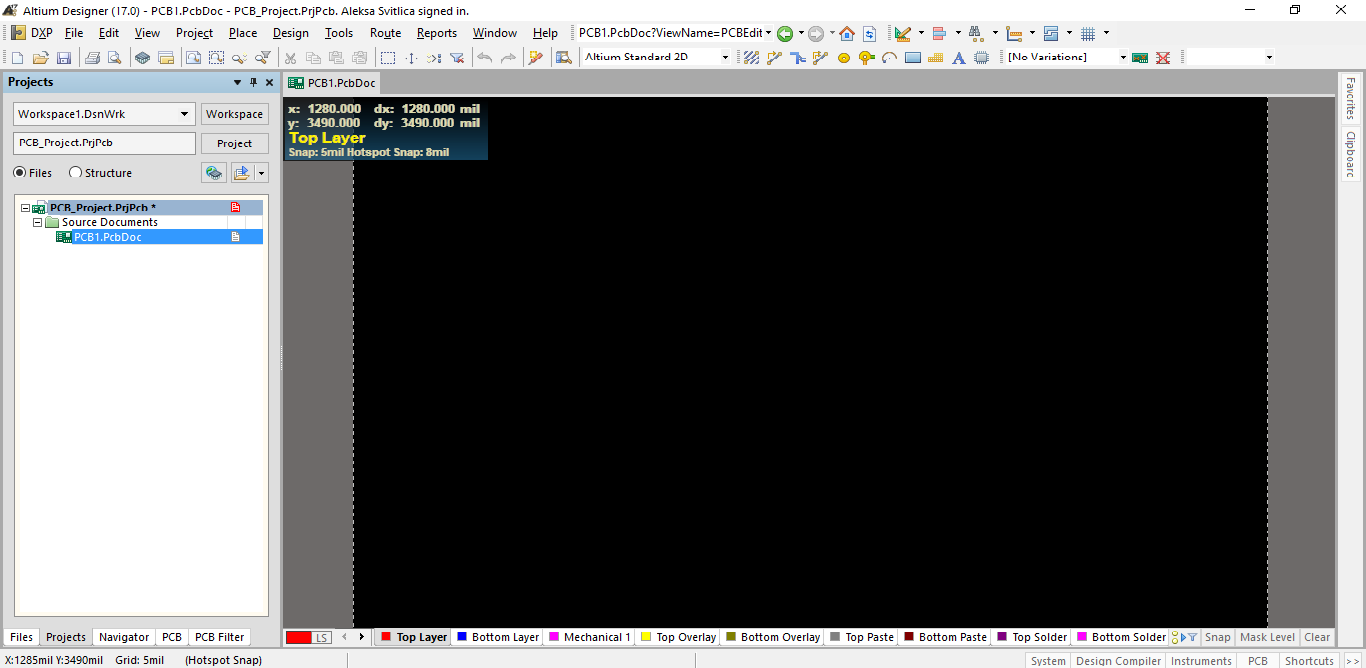
\includegraphics[width=16cm, height=8cm]{new_pcb_file.png}
		\caption{New PCB file.}
		\label{fig 1}
	\end{figure}
	The next step is import our step file and use that to create the physical PCB shape. To do this first click 3 to switch to 3D mode, you can switch between 2D and 3D by pressing 2 or 3. Then click Place-$>$3D Body to bring up a new menu. In this menu there are a couple things we need to change:
	\begin{itemize}
		\item 3D Model Type: Select Generic 3D model
		\item Further down the window there will now be an option to select a file to import for the generic 3D model. Select embedded and then choose the correct STEP file provided to you by the mechanical team.
		\item After loading your STEP file there should be a model displayed in the window, if it looks like a horizontal line don't worry, we just need to rotate it. In rotation x simple put 90 or -90.
	\end{itemize}
	\begin{figure}[H]	
		\centering
		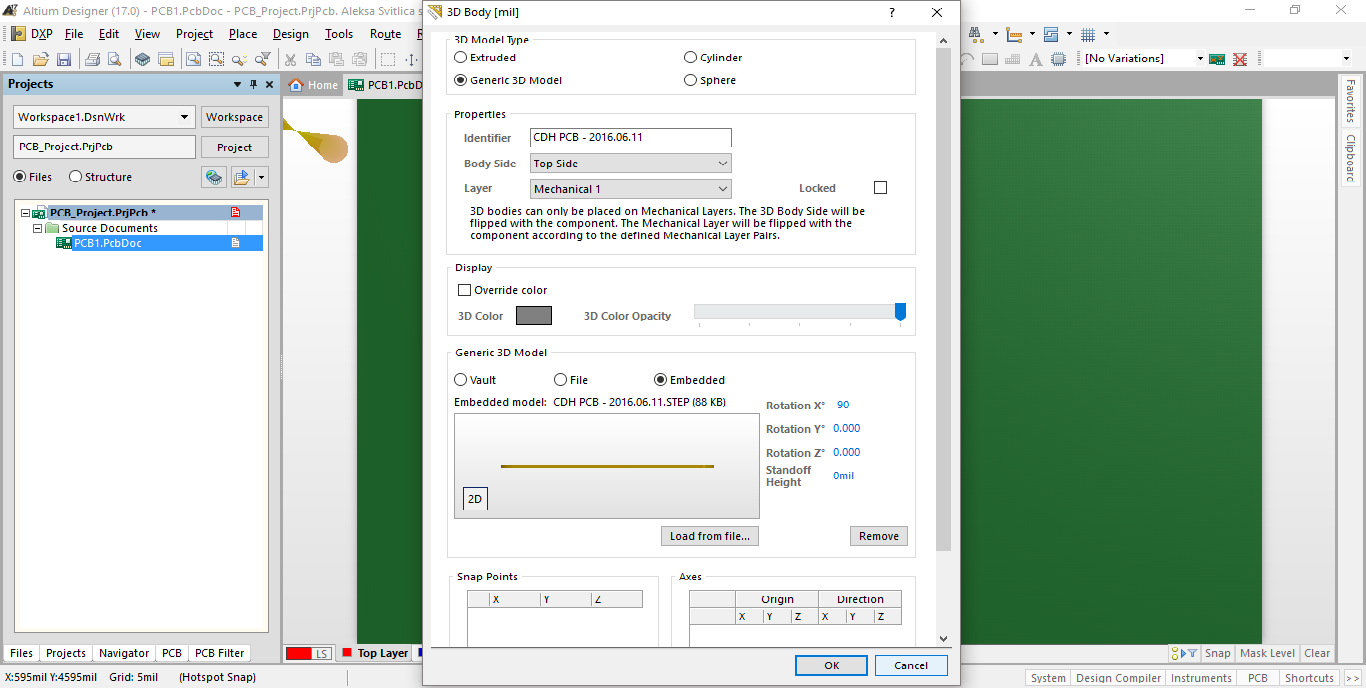
\includegraphics[width=16cm, height=8cm]{import_step.png}
		\caption{Importing STEP file as 3D body.}
		\label{fig 2}
	\end{figure}
	Click OK and left click again to place your 3D body down, where you place it doesn't matter for now.
	\begin{figure}[H]	
		\centering
		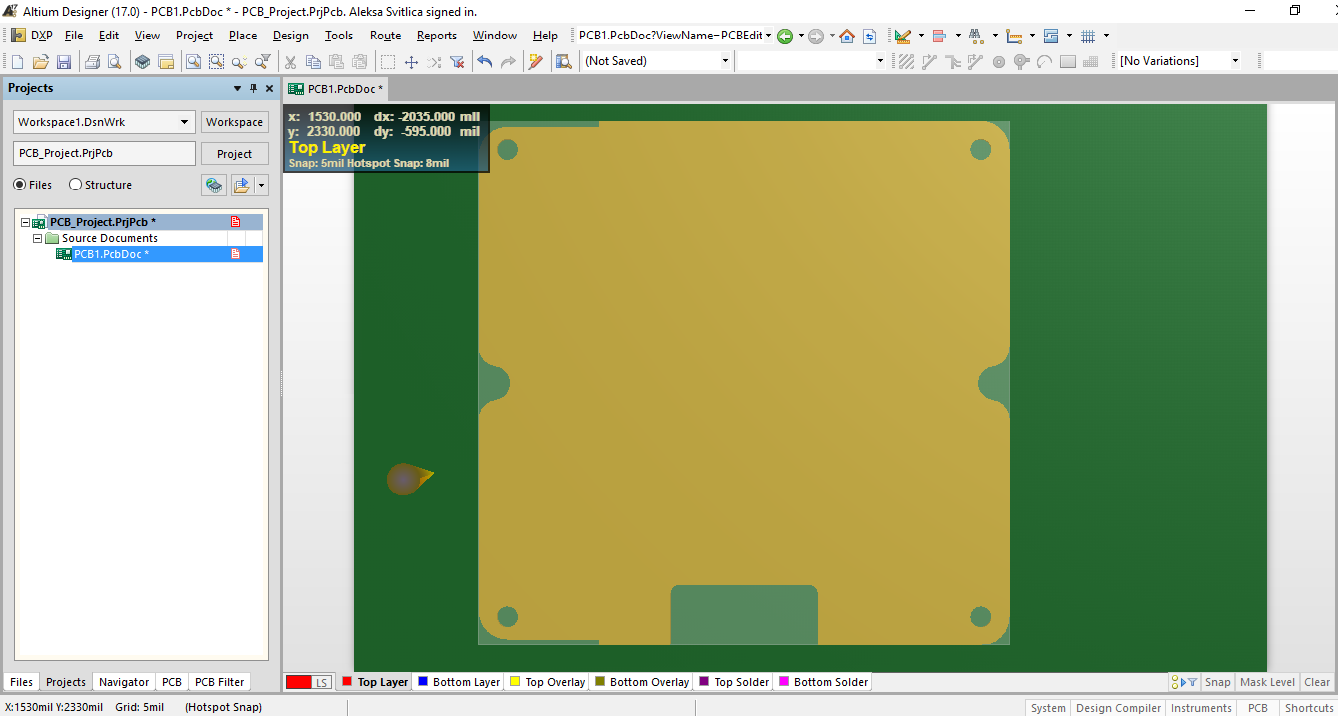
\includegraphics[width=16cm, height=8cm]{3d_body_pic1.png}
		\caption{Placing 3D body.}
		\label{fig 3}
	\end{figure}
	Now to make your PCB match this 3D body go to Design-$>$Board Shape-$>$Define From 3D Body. If this is option is unclickable for you make sure you are in 3D mode and try again. Your cursor should look like a + symbol and that window which says Top Layer in bold yellow words should also say Pick a 3D Body.
	\begin{figure}[H]	
		\centering
		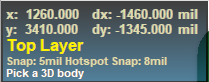
\includegraphics[width=8cm, height=4cm]{pick_3d_body.png}
		\caption{Pick 3D body.}
		\label{fig 4}
	\end{figure}
	Click on the 3D body you just placed, the words in that window should now say select face, click again on the 3D body. It will open up a couple windows, just click cancel or closed until you see the following screen.

	\begin{figure}[H]	
		\centering
		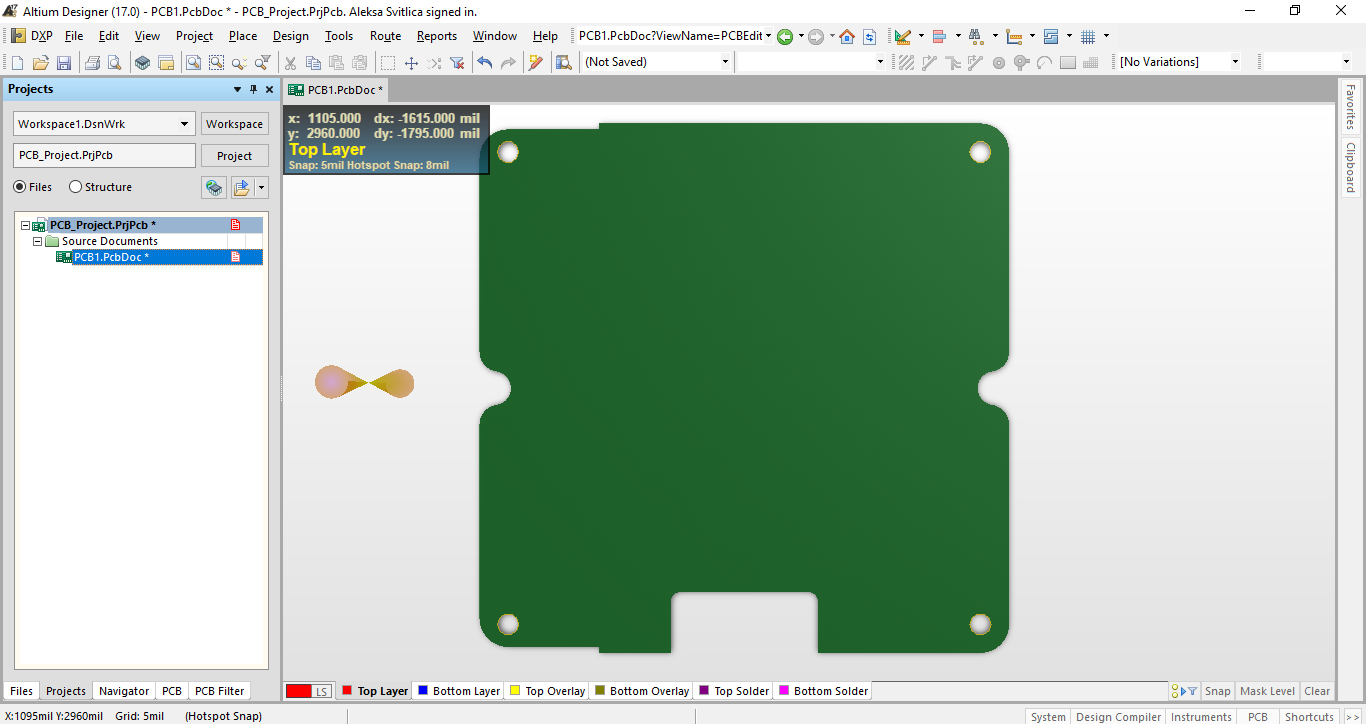
\includegraphics[width=16cm, height=8cm]{3d_body_pic2.png}
		\caption{Finished placing 3D body.}
		\label{fig 5}
	\end{figure}

	The PCB shape is now defined, we are ready to define layers.
	
	\subsection{Layer Stack Manager}
	To access the layer stack manager, select Design-$>$Layer Stack Manager. Here you can define each layer of your PCB, it will default to a 2 layer setup. Even though you see a bunch of layers listed, only the copper layers actually count when we say 2-layer board. I can't offer any suggestions about how many layers you should use, what thickness or what material since this is a topic I know almost nothing about. For reference I've included a picture of the 4-layer subsystems board that Mike Lambeta designed.
	
	\begin{figure}[H]	
		\centering
		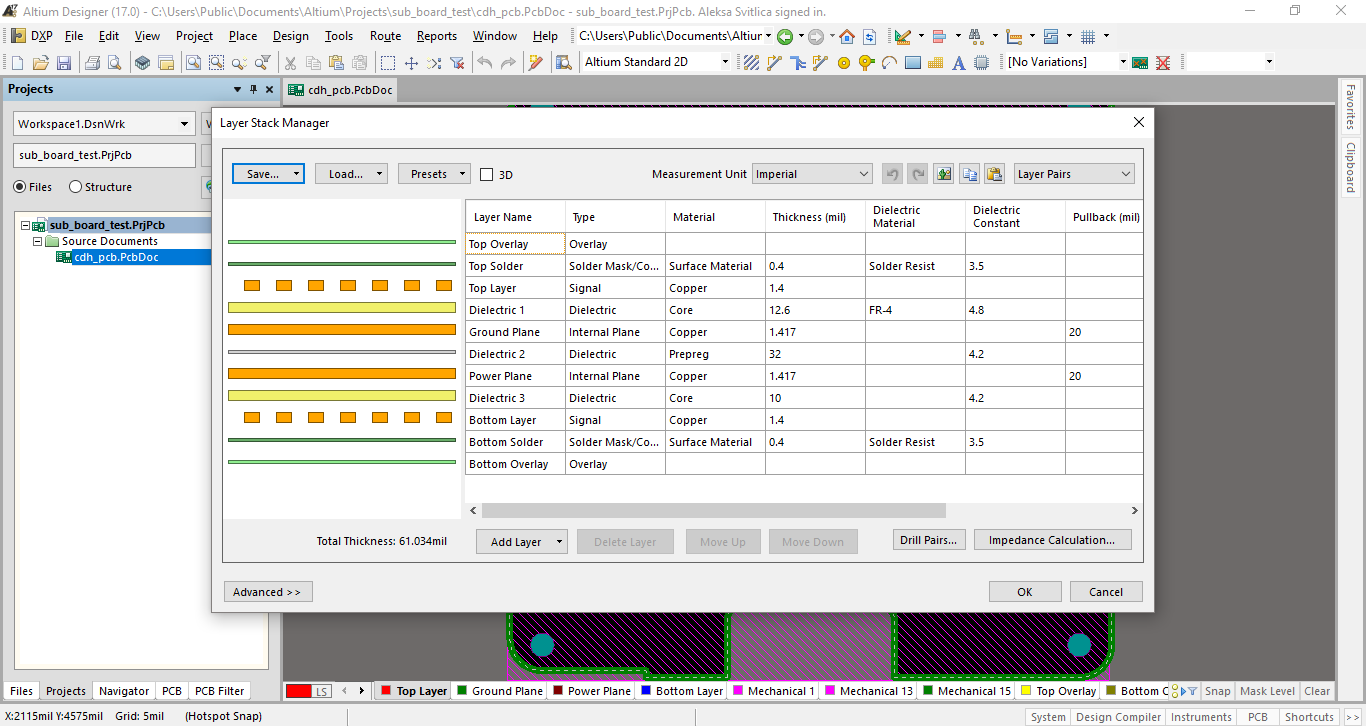
\includegraphics[width=16cm, height=8cm]{layer_stack.png}
		\caption{Layer stack manager.}
		\label{fig 6}
	\end{figure}
	
	\subsection{Parts Libraries}
	\subsubsection{Importing}
	I would recommend downloading the libraries Altium provides on their \href{http://techdocs.altium.com/display/ADOH/Download+Libraries}{website}. It is much easier to work with preexisting models since making components is a hassle. You can store the libraries anywhere on your computer and import the ones you need in your project. Click on Place-$>$Part... and then select Choose. This will bring up a menu like in the picture below, click on the three dots to the left of find. bring up the library import menu. After importing, the libraries will be selectable in the menu seen below and individual parts can be selected.
	\begin{figure}[H]	
		\centering
		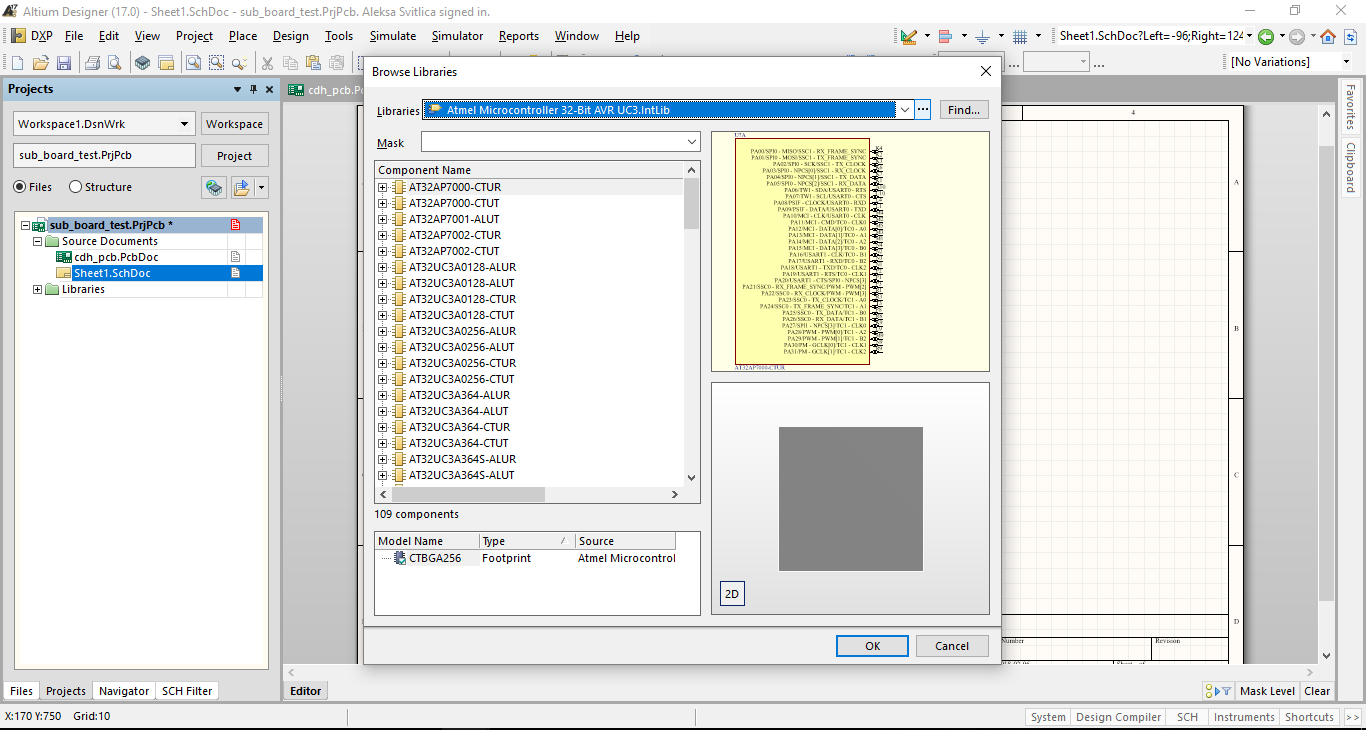
\includegraphics[width=16cm, height=8cm]{library.png}
		\caption{Browsing libraries.}
		\label{fig 7}
	\end{figure}

	\subsubsection{Custom}
	\newpage
	\section{Making Schematics}
	\section{Routing}
	
\end{document}